% !TeX root = digital-platform-api-economy.tex
% !TeX encoding = UTF-8
\chapter{Gaya API dan Pola Integrasi}
\label{ch:ch05}

% Kolom rata kiri untuk tabel bab ini: U selebar sisa tabel, V selebar yang ditentukan.
\newcolumntype{U}{>{\raggedright\arraybackslash}X}
\newcolumntype{V}[1]{>{\raggedright\arraybackslash}p{#1}}
\hyphenation{Cloud-Events}

\section*{Tujuan Pembelajaran}
\begin{itemize}
  \item Membedakan REST (\textit{Representational State Transfer}), GraphQL, \textit{event}, dan \textit{webhook} berdasarkan cara kerja dan kegunaannya.
  \item Menilai kecocokan gaya API untuk suatu kebutuhan bisnis beserta \textit{tradeoff}-nya.
  \item Memetakan integrasi yang berjalan beserta gaya dan titik masalahnya.
\end{itemize}

\section{Pendahuluan}

Bab 4 ditutup dengan inventaris sepuluh baris yang mewakili 100 sambungan. Daftar itu menjawab apa yang
tersambung dan siapa pemiliknya. Daftar itu belum menjawab siapa yang menunggu siapa, dan apa yang terjadi
ketika satu sistem gagal. Dua keluhan di Medikara Health memperlihatkan pentingnya pertanyaan itu. Klinik mitra
berulang kali menanyakan hasil laboratorium karena pemberitahuan belum tersedia. Pada saat yang sama, aplikasi
pasien Medikara+ lambat karena menunggu banyak sistem lain. Pertanyaan kemudian muncul: apakah kedua keluhan itu
masalah server yang kurang cepat, atau masalah cara sistem berkomunikasi?

Bab ini menjawabnya lewat pilihan gaya \textit{Application Programming Interface} (API) dan pola integrasi.
Pilihan itu memengaruhi waktu tunggu, ketergantungan, dan cara organisasi menangani kegagalan. Bahasannya meliputi
empat cara sistem bertukar data, komunikasi sinkron dan asinkron, REST, GraphQL, \textit{event} dan
\textit{webhook}, lalu kriteria memilih gaya API dengan gRPC sebagai pembanding singkat. Arsitektur berbasis
\textit{event} hanya disinggung, karena dibahas rinci di IT40713 Cloud-Native \& Microservices Architecture. Angka
tambahan yang diawali kata ``Misalkan'' adalah asumsi latihan. Kesimpulan untuk organisasi nyata harus diuji dengan
wawancara, dokumen, dan pengukuran yang berizin. Hasil bab ini menjadi bagian tonggak C2 dalam cetak biru
transformasi digital.

Rujukan utama bab ini dipakai untuk membedakan konsep dan membangun alasan keputusan, bukan untuk menggantikan
penilaian konteks organisasi. Empat cara bertukar data diambil dari Hohpe dan Woolf \cite{c05-hohpe2003eip}. Gaya
REST diambil dari disertasi Fielding \cite{c05-fielding2000rest}, sedangkan arti metode dan kode status diambil
dari \textit{Request for Comments} (RFC) 9110 \cite{rfc9110}. GraphQL mengikuti spesifikasi resminya \cite{c05-graphql-spec}. Pola pertukaran data
API diambil dari Zimmermann dkk. \cite{zimmermann2022patterns}. Format kontrak OpenAPI \cite{openapi32} dan
AsyncAPI \cite{asyncapi31} hanya disebut di sini, karena dibahas di Bab 9.

\IfFileExists{../figures/ch05-diagram-konsep.png}{%

Gambar \ref{fig:ch05-ilustrasi-bab} merangkum hubungan komponen dan konsep utama bab ini.
\begin{figure}[!htb]
  \centering
  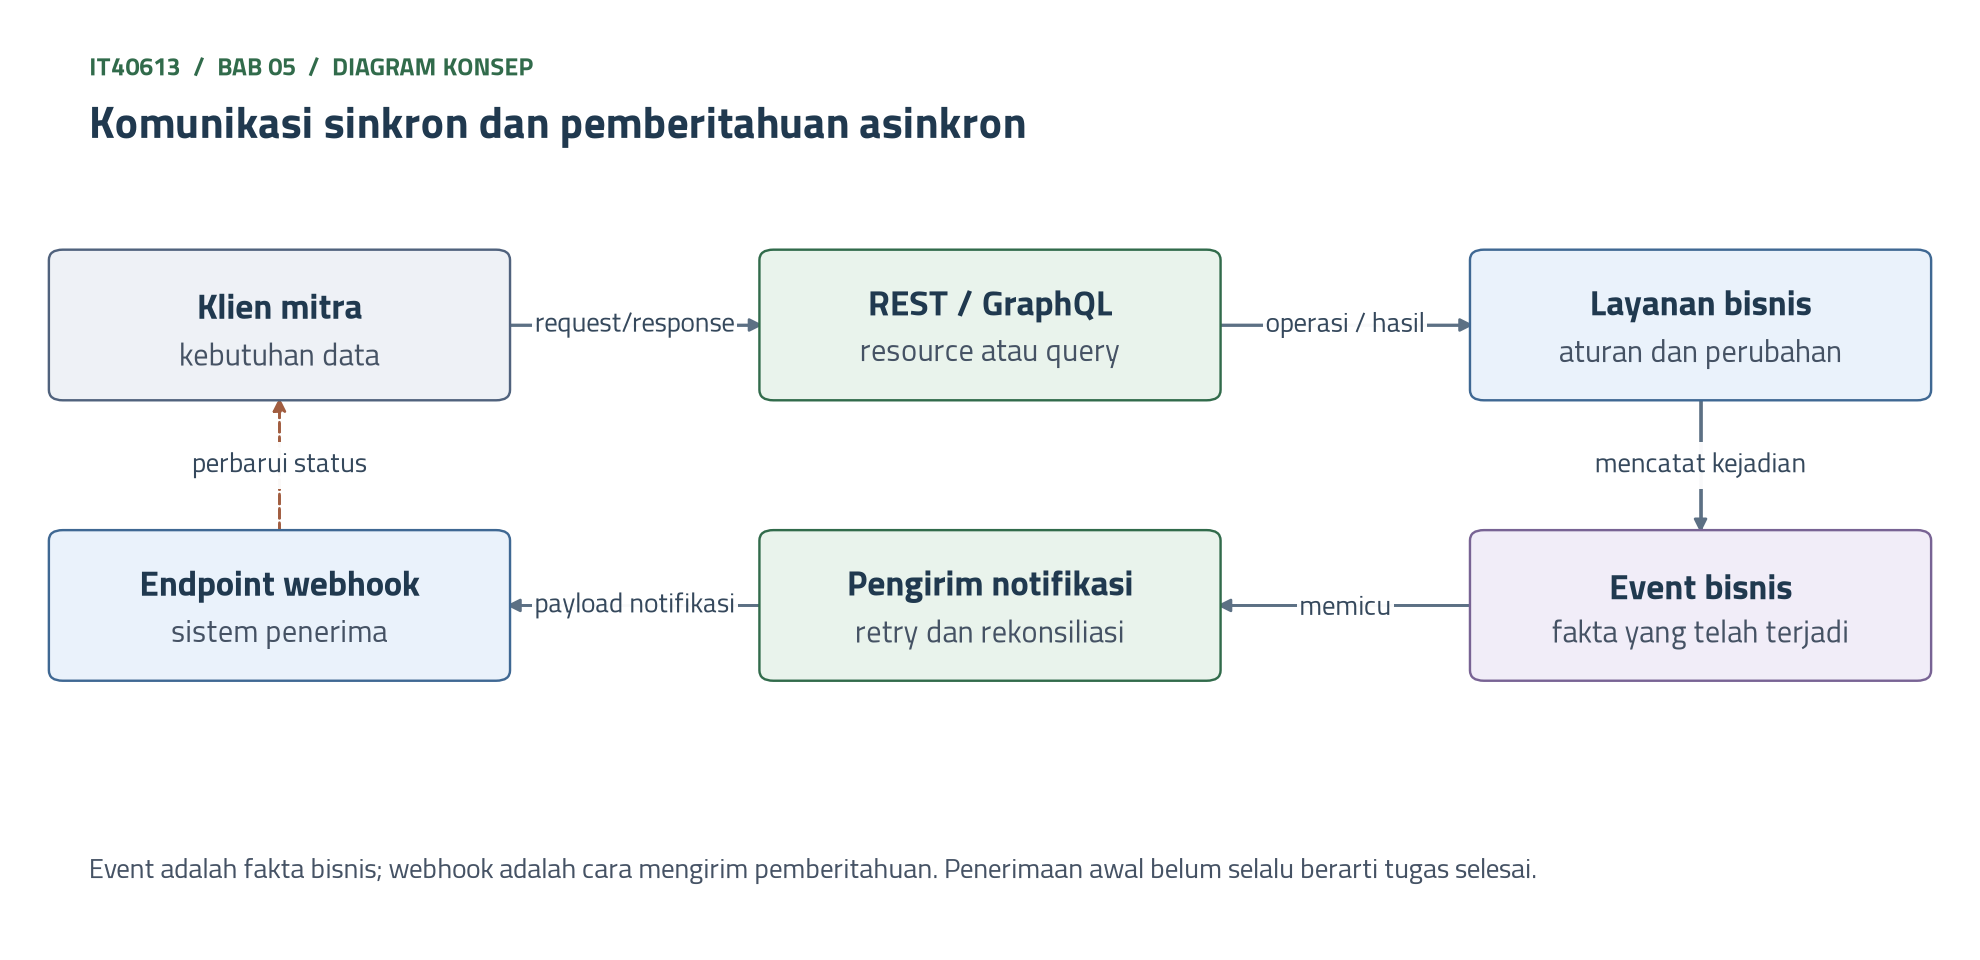
\includegraphics[width=\textwidth]{../figures/ch05-diagram-konsep.png}
  \caption{Komunikasi sinkron dan pemberitahuan asinkron}
  \label{fig:ch05-ilustrasi-bab}
\end{figure}
}{}

\section{Empat Cara Sistem Bertukar Data}

Kolom cara pertukaran pada inventaris Bab 4 berisi banyak istilah: API, ekspor berkas, portal, surel, dan akses
langsung ke basis data. Pertanyaannya, dapatkah istilah sebanyak itu diringkas supaya pilihannya terlihat?

Hohpe dan Woolf meringkas pendekatan integrasi aplikasi menjadi empat gaya utama \cite{c05-hohpe2003eip}. Pada
pertukaran berkas (\textit{file transfer}), satu aplikasi menghasilkan berkas dan aplikasi lain membacanya. Data
terkumpul dulu, lalu diproses pada waktu tertentu. Pada basis data bersama (\textit{shared database}), beberapa
aplikasi menyimpan data yang dibagi di satu basis data. Akses menjadi mudah, tetapi semua pemakai bergantung pada
struktur yang sama. Pada panggilan langsung (\textit{remote procedure invocation}), satu aplikasi membuka sebagian
kemampuannya agar dapat dipanggil dari jauh, sehingga jawaban datang segera. Pada pesan (\textit{messaging}),
aplikasi tersambung ke sistem pesan bersama, sehingga waktu pengirim dan penerima terpisah. Keempatnya dapat hidup
bersama dalam satu organisasi, asalkan kepemilikan dan akibat kegagalannya jelas.

Analoginya koordinasi di kantor. Laporan harian diletakkan di meja atasan setiap sore. Lemari arsip dipakai semua
bagian, tetapi ketika satu bagian mengganti cara menyusun map, bagian lain kebingungan. Telepon memberi jawaban saat
itu juga, selama orang di ujung sana ada. Kotak surat menerima pesan kapan saja, walaupun penerimanya sedang keluar.

Dua contoh penerapan pada Medikara:
\begin{enumerate}
  \item Pertukaran berkas pada INT-05. Tagihan dan dokumen klaim diunggah ke portal 9 asuransi setiap minggu,
        dengan 7.800 klaim per bulan. Cara ini cocok bila proses memang berbasis periode. Misalkan klaim muncul
        merata sepanjang minggu. Satu klaim rata-rata menunggu 3,5 hari sebelum diunggah. Penolakan karena format,
        yaitu 468 klaim per bulan, baru diketahui sesudah unggahan. Perubahan status yang dibutuhkan dalam hitungan
        menit memerlukan mekanisme lain.
  \item Basis data bersama pada INT-03. Menurut Bab 1, vendor Medikara+ membaca basis data Sistem Informasi
        Manajemen Rumah Sakit (SIMRS) di tiga rumah sakit setiap lima menit, sedangkan dua rumah sakit lain dipanggil lewat
        API bawaan. Itu berarti 288 pembacaan per hari per rumah sakit, atau 864 per hari untuk ketiganya. Bab 1
        juga memisalkan tujuh kali pembaruan SIMRS sepanjang 2025, dan tiap pembaruan membuat jadwal kosong satu
        sampai dua hari. Akibatnya jadwal kosong 7 sampai 14 hari dalam setahun. Bila mitra diizinkan menulis
        langsung ke tabel SIMRS, aturan bisnis seperti pemeriksaan slot bahkan dapat terlewati. Antarmuka layanan
        membatasi operasi dan mengurangi ketergantungan pada struktur tabel.
\end{enumerate}

Tabel \ref{tab:ch05-empat-cara} merangkum kekuatan dan risiko keempat cara itu. Contoh panggilan langsung diambil dari INT-01, yaitu
sambungan ke Badan Penyelenggara Jaminan Sosial (BPJS) Kesehatan.

\begin{table}[!htb]
  \centering
  \caption{Empat cara sistem bertukar data, dengan contoh dari inventaris Medikara}
  \label{tab:ch05-empat-cara}
  \footnotesize
  \begin{tabularx}{\textwidth}{V{2.0cm}UUV{2.5cm}}
    \hline
    \textbf{Cara} & \textbf{Kekuatan} & \textbf{Risiko} & \textbf{Contoh Medikara} \\ \hline
    Pertukaran berkas & Sederhana, cocok untuk kiriman berkala dalam jumlah besar & Jeda pengiriman, salah format baru terlihat belakangan & INT-05: klaim mingguan ke 9 portal \\ \hline
    Basis data bersama & Data tersedia tanpa perantara & Pemakai terikat pada struktur tabel, akses mudah melebar & INT-03: 140 tabel terbaca, 2 tabel dibutuhkan \\ \hline
    Panggilan langsung & Jawaban segera, kesalahan langsung terlihat & Pemanggil bergantung pada ketersediaan penyedia & INT-01: kepesertaan BPJS Kesehatan per kunjungan \\ \hline
    Pesan & Pengirim dan penerima tidak perlu hidup bersamaan & Pengolahan tertunda, perlu pelacakan dan penanganan pesan ganda & Belum ada, hasil laboratorium menjadi calon \\ \hline
  \end{tabularx}
\end{table}

Inventaris Bab 4 dapat dibaca ulang dengan empat cara tersebut. Tabel \ref{tab:ch05-sebaran} menghitungnya per
sambungan. Surel berisi hasil pindaian dan \textit{spreadsheet} dihitung sebagai pertukaran berkas, karena yang
berpindah adalah berkas, dan manusia yang membaca atau mengetik ulang isinya.

\begin{table}[!htb]
  \centering
  \caption{Sepuluh baris inventaris Medikara menurut empat cara bertukar data: 85 dari 100 sambungan memakai berkas}
  \label{tab:ch05-sebaran}
  \small
  \begin{tabularx}{\textwidth}{V{3.9cm}UV{1.8cm}}
    \hline
    \textbf{Cara} & \textbf{Baris inventaris} & \textbf{Sambungan} \\ \hline
    Pertukaran berkas & INT-04, INT-05, INT-06, INT-07, INT-08, INT-09, INT-10 & 85 \\ \hline
    Basis data bersama & INT-03 & 5 \\ \hline
    Panggilan langsung & INT-01, INT-02 & 10 \\ \hline
    Pesan & Belum ada & 0 \\ \hline
    \textbf{Jumlah} & 10 baris & \textbf{100} \\ \hline
  \end{tabularx}
\end{table}

Baris INT-03 dihitung menurut cara yang dominan, yaitu basis data bersama pada tiga dari lima sambungan. Dua sambungan lain
memakai API bawaan, seperti dicatat inventaris Bab 4. Hitungan ini punya dua konsekuensi. Pertama, 85 persen sambungan bergerak mengikuti jadwal
pengiriman, sehingga janji ``segera'' kepada mitra belum mungkin dipenuhi. Kedua, belum ada satu pun sambungan
berbasis pesan, sehingga pihak yang menunggu perubahan hanya dapat bertanya berulang. Keluhan klinik mitra berasal
dari sini.

Dua hal pada bahasan ini sering tertukar, yaitu cara bertukar data dan gaya API. Pembagiannya begini. Cara bertukar
data menjawab lewat jalur apa data berpindah. Gaya API menjawab bagaimana kontrak antarmuka dibentuk. REST, GraphQL,
dan gRPC termasuk panggilan langsung. \textit{Event} biasanya diantar lewat pesan atau \textit{webhook}. Karena itu,
jawaban ``sudah memakai API'' dalam wawancara belum menjelaskan siapa menunggu siapa. Pertanyaan berikutnya
langsung mengarah ke sana.

\section{Komunikasi Sinkron dan Asinkron}

Pada komunikasi sinkron, pemanggil menunggu jawaban dalam satu interaksi. Pada komunikasi asinkron, penerimaan
permintaan dan penyelesaian pekerjaan terjadi pada waktu berbeda. Asinkron tidak menjamin pekerjaan selesai, sehingga
diperlukan identitas pekerjaan, status, tenggat, dan penanganan kegagalan. Ketersediaan juga bergantung pada
keseluruhan rantai, bukan hanya layanan pertama yang dipanggil. Gambar \ref{fig:ch05-sinkron-asinkron} menyandingkan
kedua pola itu.

\begin{figure}[!htb]
  \centering
  \begin{tikzpicture}[
  font=\scriptsize,
  execute at begin node={\hyphenpenalty=10000\exhyphenpenalty=10000},
  aktor/.style={draw, rounded corners, fill=blue!8, minimum width=1.6cm, minimum height=0.6cm, align=center},
  judul/.style={font=\scriptsize\bfseries, align=center},
  garis/.style={dashed, gray},
  ket/.style={font=\tiny, align=center},
  panah/.style={-{Stealth[length=2mm]}, thick},
  balik/.style={-{Stealth[length=2mm]}, thick, dashed}
]
  % Panel kiri: pemanggil menunggu sepanjang penyedia bekerja.
  \node[judul] at (2.6,0.75) {Sinkron: pemanggil menunggu jawaban};
  \node[aktor] (pa) at (0.8,0) {Pemanggil};
  \node[aktor] (sa) at (4.4,0) {Penyedia};
  \draw[garis] (pa.south) -- (0.8,-4.3);
  \draw[garis] (sa.south) -- (4.4,-4.3);
  \draw[fill=red!22] (0.68,-0.8) rectangle (0.92,-3.3);
  \draw[fill=orange!12] (4.28,-0.8) rectangle (4.52,-3.3);
  \draw[panah] (0.92,-0.8) -- node[above, ket] {\textit{request}} (4.28,-0.8);
  \node[ket, anchor=west] at (1.0,-1.7) {pemanggil tertahan};
  \node[ket, anchor=east] at (4.2,-2.4) {penyedia bekerja};
  \draw[balik] (4.28,-3.3) -- node[above, ket] {\textit{response}: 200 dan hasil} (0.92,-3.3);
  \node[ket] at (2.6,-3.85) {Hasil tiba dalam satu interaksi};
  \node[ket] at (2.6,-4.6) {Bila penyedia lambat, pemanggil ikut lambat};

  % Panel kanan: penerimaan dan penyelesaian terjadi pada waktu berbeda.
  \begin{scope}[xshift=6.4cm]
    \node[judul] at (2.6,0.75) {Asinkron: diterima dulu, selesai belakangan};
    \node[aktor] (pb) at (0.8,0) {Pemanggil};
    \node[aktor] (sb) at (4.4,0) {Penyedia};
    \draw[garis] (pb.south) -- (0.8,-4.3);
    \draw[garis] (sb.south) -- (4.4,-4.3);
    \draw[fill=red!22] (0.68,-0.8) rectangle (0.92,-1.3);
    \draw[fill=orange!12] (4.28,-0.8) rectangle (4.52,-3.6);
    \draw[panah] (0.92,-0.8) -- node[above, ket] {\textit{request}} (4.28,-0.8);
    \draw[balik] (4.28,-1.3) -- node[above, ket] {202 dan ID pekerjaan} (0.92,-1.3);
    \node[ket, anchor=west] at (1.0,-1.75) {pemanggil mengerjakan hal lain};
    \draw[panah] (0.8,-2.45) -- node[above, ket] {tanya status memakai ID} (4.28,-2.45);
    \draw[balik] (4.28,-2.85) -- node[above, ket] {masih diproses} (0.8,-2.85);
    \draw[balik, draw=praditagreen] (4.28,-3.6) -- node[above, ket] {selesai atau gagal} (0.8,-3.6);
    \node[ket] at (2.6,-4.6) {Jawaban pertama hanya berarti ``diterima'', bukan ``selesai''};
  \end{scope}
\end{tikzpicture}

  \caption{Pada pola sinkron pemanggil tertahan sampai hasil tiba, sedangkan pada pola asinkron jawaban pertama hanya berarti permintaan diterima}
  \label{fig:ch05-sinkron-asinkron}
\end{figure}

Analoginya telepon dan surat. Telepon meminta perhatian saat itu juga, dan penelepon tidak dapat mengerjakan hal lain
sampai pembicaraan selesai. Bila yang ditelepon tidak mengangkat, pekerjaan berhenti. Surat memberi jeda, sehingga
pengirim dapat bekerja lagi. Namun surat perlu alamat, bukti terima, dan cara melacak bila balasan tidak kunjung
datang.

Dua contoh berangka memperlihatkan akibatnya:
\begin{enumerate}
  \item Misalkan pemesanan di Medikara+ menunggu layanan notifikasi selama lima detik. Dengan 28.000 janji temu per
        bulan, pasien kehilangan 140.000 detik, atau sekitar 39 jam per bulan, hanya untuk menunggu pengingat yang
        tidak perlu ditunggu. Misalkan pula ketersediaan API janji temu 99,9 persen, SIMRS 99,5 persen, dan layanan
        notifikasi 99,0 persen, dengan kegagalan yang saling lepas. Bila ketiganya dirangkai sinkron, ketersediaan
        rantai menjadi 98,41 persen, sehingga sekitar 446 pemesanan per bulan gagal. Bila notifikasi dipisah menjadi
        asinkron, ketersediaan rantai menjadi 99,40 persen, dan yang gagal sekitar 168 pemesanan. Gangguan notifikasi
        tidak lagi menghambat transaksi yang sudah dapat disimpan.
  \item Misalkan rekap INT-07 bagi 36 perusahaan klien sudah otomatis, dan satu rekap butuh 3 menit, sehingga semuanya
        butuh 108 menit. Misalkan batas waktu panggilan 30 detik. Panggilan sinkron selalu gagal, walaupun rekapnya
        benar. Permintaan pembuatan rekap sebaiknya diterima dengan kode 202 dan ID pekerjaan. Pengguna kemudian
        memeriksa apakah statusnya selesai atau gagal.
\end{enumerate}

Dua hal pada komunikasi asinkron sering tertukar, yaitu diterima dan selesai. Pembagiannya begini. RFC 9110 menjelaskan
kode 202 sebagai permintaan yang diterima untuk diproses, tetapi prosesnya belum selesai. Permintaan itu mungkin saja
tidak pernah dijalankan. Standar yang sama menyebut \textit{HyperText Transfer Protocol} (HTTP) tidak punya sarana
untuk mengirim ulang kode status dari operasi asinkron \cite{rfc9110}. Karena itu ID pekerjaan dan \textit{endpoint}
status harus dirancang, bukan dianggap otomatis tersedia. Tabel \ref{tab:ch05-sinkron-asinkron} merangkum perbedaan
yang perlu diperiksa.

\begin{table}[!htb]
  \centering
  \caption{Komunikasi sinkron dan asinkron berbeda pada arti jawaban pertama dan akibat kegagalan}
  \label{tab:ch05-sinkron-asinkron}
  \small
  \begin{tabularx}{\textwidth}{V{2.9cm}UU}
    \hline
    \textbf{Unsur} & \textbf{Sinkron} & \textbf{Asinkron} \\ \hline
    Arti jawaban pertama & Hasil akhir & Permintaan diterima \\ \hline
    Bila penyedia mati & Pemanggil langsung gagal & Pekerjaan tertunda, pemanggil tetap berjalan \\ \hline
    Saat beban puncak & Pemanggil ikut melambat & Antrean memanjang, perlu dipantau \\ \hline
    Yang wajib disediakan & Batas waktu yang jelas & ID pekerjaan, status, tenggat, dan eskalasi \\ \hline
    Contoh Medikara & Konfirmasi slot dokter & Pembuatan rekap, pengingat, hasil tersedia \\ \hline
  \end{tabularx}
\end{table}

Apakah semua sebaiknya asinkron? Tidak. Konfirmasi slot harus dijawab segera, karena pasien memutuskan berangkat
berdasarkan jawaban itu. Misalkan konfirmasi dijadikan asinkron dan 1 persen pemesanan ternyata bentrok. Sebanyak 280
pasien per bulan sudah menerima kabar berhasil, lalu diberi tahu bahwa slotnya hilang. Yang diuji pada setiap langkah
adalah apakah orang atau sistem berikutnya benar-benar tidak dapat lanjut tanpa jawaban.

\begin{kasus}[title={Kasus Medikara Health: Aplikasi Pasien yang Menunggu Semua Pihak}]
Bab 4 mencatat tiga panggilan per pemesanan, sehingga 28.000 janji temu menghasilkan 84.000 panggilan per bulan. Tim
menelusuri langkah pemesanan dan menandai langkah yang benar-benar wajib dijawab saat itu juga.
\begin{enumerate}
  \item Wajib sinkron: mencari jadwal, memilih slot, dan mengunci slot. Tanpa jawaban, pasien tidak dapat memutuskan.
  \item Boleh asinkron: pengingat, pesan konfirmasi ke surel, dan pencatatan untuk laporan. Pemesanan sudah sah tanpa
        ketiganya.
\end{enumerate}

Keputusan ini punya dua konsekuensi. Pertama, ketersediaan rantai pemesanan naik dari 98,41 persen menjadi 99,40
persen pada asumsi tadi, atau sekitar 278 pemesanan per bulan yang tidak lagi gagal. Kedua, Medikara menanggung
pekerjaan baru: pengingat yang gagal harus dikirim ulang, dan pasien yang tidak menerima pengingat tetap harus dapat
melihat janjinya di aplikasi. Pemilik keputusan ini adalah Manajer Layanan Rawat Jalan, karena ia yang merasakan akibat
antrean.
\end{kasus}

\section{REST: Sumber Daya, Metode, dan Kode Status}

Bila jawaban memang dibutuhkan segera, bagaimana kontrak panggilan langsung sebaiknya dibentuk? Gaya pertama yang
dibahas adalah REST.

REST adalah gaya arsitektur untuk sistem hipermedia terdistribusi, bukan sekadar penamaan \textit{Uniform Resource
Locator} (URL). Fielding membangunnya dari sederet batasan: klien dan server dipisah, setiap permintaan berdiri sendiri tanpa
bergantung pada keadaan sesi di server, jawaban dapat disimpan di \textit{cache}, antarmuka seragam, sistem berlapis, dan
kode sesuai permintaan yang bersifat opsional. Abstraksi utamanya adalah sumber daya (\textit{resource}), yaitu informasi
apa pun yang dapat diberi nama \cite{c05-fielding2000rest}. Banyak API yang menyebut dirinya REST hanya mengambil sebagian
batasan itu. Bab ini memakai istilah REST untuk praktik HTTP yang memakai sumber daya, metode, kode status, dan semantik
pengulangan secara konsisten. Kontraknya biasa ditulis dengan OpenAPI, yang mendeskripsikan API HTTP secara baku
\cite{openapi32}.

Metode HTTP membawa janji tentang akibatnya. RFC 9110 menyebut metode aman (\textit{safe}) bila maknanya pada dasarnya
hanya membaca, sehingga klien tidak meminta perubahan keadaan di server. Metode disebut idempoten bila efek yang dimaksud
dari beberapa permintaan identik sama dengan efek satu permintaan \cite{rfc9110}. \texttt{GET} aman dan idempoten.
\texttt{PUT} dan \texttt{DELETE} idempoten. \texttt{POST} tidak aman dan tidak idempoten, sehingga memerlukan rancangan
tambahan bila pengulangan dapat membuat transaksi ganda. Tabel \ref{tab:ch05-metode} merangkumnya.

\begin{table}[!htb]
  \centering
  \caption{Metode HTTP membawa janji tentang akibat dan pengulangan}
  \label{tab:ch05-metode}
  \small
  \begin{tabularx}{\textwidth}{V{1.4cm}UV{1.0cm}V{1.8cm}U}
    \hline
    \textbf{Metode} & \textbf{Arti} & \textbf{Aman} & \textbf{Idempoten} & \textbf{Contoh Medikara} \\ \hline
    \texttt{GET} & Membaca sumber daya & Ya & Ya & Membaca jadwal dokter \\ \hline
    \texttt{POST} & Memproses permintaan, sering membuat data baru & Tidak & Tidak & Membuat janji temu \\ \hline
    \texttt{PUT} & Mengganti keadaan sumber daya & Tidak & Ya & Mengganti data kontak pasien \\ \hline
    \texttt{DELETE} & Menghapus sumber daya & Tidak & Ya & Membatalkan janji temu \\ \hline
  \end{tabularx}
\end{table}

Analoginya formulir di loket layanan. Formulir yang berbeda dipakai untuk membaca jadwal, membuat pemesanan, dan
membatalkan pemesanan. Petugas mengetahui maksudnya dari jenis formulir, tanpa harus membaca seluruh isinya. Jawabannya
berupa cap yang artinya sama di semua loket. Pemohon yang menerima cap ``slot sudah terisi'' tahu ia harus memilih slot
lain, bukan mengantre ulang.

Dua contoh penerapan pada Medikara:
\begin{enumerate}
  \item \texttt{GET /jadwal-dokter} dari Bab 1 mengembalikan 200 bila pencarian berhasil. Hasil kosong dapat berupa
        daftar kosong, bukan otomatis kesalahan sistem. Misalkan dari tiga panggilan per pemesanan, dua membaca dan satu
        membuat janji, sehingga ada 56.000 \texttt{GET} dan 28.000 \texttt{POST} per bulan. Karena \texttt{GET} aman,
        jawabannya dapat disimpan di \textit{cache}. Misalkan separuh pembacaan dilayani \textit{cache} lima menit. SIMRS
        terhindar dari 28.000 pembacaan per bulan.
  \item \texttt{POST /janji-temu} dapat menghasilkan 201 beserta lokasi sumber daya baru. Misalkan pada 1 persen pemesanan,
        yaitu 280 per bulan, jawaban hilang di jaringan, lalu aplikasi mengirim ulang. Misalkan separuhnya sudah tersimpan
        pada kiriman pertama, sehingga muncul 140 janji ganda per bulan. Dengan 6 menit per perbaikan, biayanya 14 jam per
        bulan, atau Rp10,08 juta per tahun pada tarif Rp60.000 per jam. Pengulangan sebaiknya memakai kunci idempotensi
        sesuai kontrak agar tidak membuat dua janji.
\end{enumerate}

Kunci idempotensi belum menjadi standar selesai. Bidang \texttt{Idempotency-Key} masih berupa draf di \textit{Internet
Engineering Task Force} (IETF). Tujuannya membuat metode tak idempoten seperti \texttt{POST} tahan terhadap gangguan
\cite{idempotency-key-draft}. Akibatnya, kontrak Medikara harus menuliskan sendiri cara memakai kunci itu dan berapa lama
kunci disimpan.

Kode status menyampaikan apa yang terjadi dan siapa yang harus bertindak. Bab 1 sudah memperkenalkan 200, 400, 401, 403,
404, 500, dan 503. Tabel \ref{tab:ch05-kode-status} menambahkan kode yang dibutuhkan bab ini. Kode 429 berasal dari RFC 6585
\cite{rfc6585}, sedangkan kode lainnya dari RFC 9110 \cite{rfc9110}.

\begin{table}[!htb]
  \centering
  \caption{Kode status tambahan pada API janji temu, hasil, dan rekap Medikara}
  \label{tab:ch05-kode-status}
  \small
  \begin{tabularx}{\textwidth}{V{0.8cm}V{2.3cm}UV{2.8cm}}
    \hline
    \textbf{Kode} & \textbf{Nama} & \textbf{Contoh Medikara} & \textbf{Yang bertindak} \\ \hline
    201 & Created & Janji temu dibuat, lokasinya ada di \textit{header} \texttt{Location} & Tidak ada \\ \hline
    202 & Accepted & Permintaan rekap diterima, prosesnya belum selesai & Pemanggil memeriksa status \\ \hline
    409 & Conflict & Slot sudah dipakai pasien lain & Pasien memilih slot lain \\ \hline
    429 & Too Many Requests & Klinik melampaui kuota 300 panggilan per hari & Klinik menunda sesuai \textit{header} \texttt{Retry-After} \\ \hline
  \end{tabularx}
\end{table}

Kode status yang dipakai sembarangan mahal akibatnya. Misalkan API menjawab 200 untuk slot yang bentrok, lalu menaruh
kata ``gagal'' di isi jawaban. \textit{Dashboard} mencatat 100 persen berhasil, padahal 280 pemesanan bentrok dalam sebulan
tidak terlihat. Kode 409 membuat kegagalan yang sama terbaca oleh aplikasi, oleh alat pemantau, dan oleh pemilik produk.

\begin{pendalaman}[title={Pendalaman Teknis (opsional): Membaca Permintaan dan Jawaban REST}]
Listing \ref{lst:ch05-rest} memperlihatkan dua panggilan pada contoh di atas. Panggilan kedua membawa kunci idempotensi
dengan bentuk yang dicontohkan draf IETF \cite{idempotency-key-draft}. Bila kiriman diulang dengan kunci yang sama, kontrak
Medikara mewajibkan server mengembalikan janji yang sudah ada, bukan membuat janji baru. Alamat dan pengenal pada contoh
ini fiktif.

\begin{lstlisting}[language=http, xleftmargin=8pt, captionpos=b, caption={Membaca jadwal dan membuat janji temu, tersedia di \berkas{sources/chapter05/contoh-rest-graphql.md}}, label={lst:ch05-rest}]
GET /jadwal-dokter?rumahSakit=bekasi&tanggal=2026-11-02 HTTP/1.1
Host: api.medikara.example
Accept: application/json

HTTP/1.1 200 OK
Content-Type: application/json
Cache-Control: max-age=300

{"rumahSakit": "bekasi", "tanggal": "2026-11-02", "slot": []}

POST /janji-temu HTTP/1.1
Host: api.medikara.example
Content-Type: application/json
Idempotency-Key: "8e03978e-40d5-43e8-bc93-6894a57f9324"

{"slot": "BKS-20261102-0915", "pasien": "PSN-58213"}

HTTP/1.1 201 Created
Location: /janji-temu/JT-40771
\end{lstlisting}
\end{pendalaman}

\section{GraphQL}

REST menetapkan bentuk jawaban di sisi penyedia. Apa yang terjadi bila tiap layar membutuhkan kombinasi data yang berbeda?

GraphQL adalah bahasa \textit{query} untuk membangun aplikasi klien, dengan sintaks untuk menggambarkan kebutuhan data dan
interaksinya. Setiap layanan GraphQL mendefinisikan sistem tipe, dan permintaan dijalankan dalam sistem tipe itu.
GraphQL bukan bahasa pemrograman, dan tidak mewajibkan bahasa atau tempat penyimpanan tertentu \cite{c05-graphql-spec}.
Klien memilih bidang yang dibutuhkan, lalu menerima jawaban dengan bentuk yang sama. Zimmermann dkk. memuat masalah yang
serupa sebagai pola Wish List: klien memberi tahu penyedia pada saat dijalankan data mana yang diminati
\cite{zimmermann2022patterns}. Artinya REST juga dapat meniru sebagian manfaat ini lewat parameter pilihan bidang. Server
GraphQL tetap menentukan otorisasi, biaya pemrosesan, dan batas kedalaman permintaan. Satu \textit{endpoint} tidak berarti
satu operasi murah.

Analoginya daftar pesanan katering. Pelanggan memilih lauk sesuai selera, tanpa harus membeli paket yang sudah ditentukan
dapur. Namun dapur tetap membatasi kapasitas dan bahan. Pesanan 40 jenis lauk untuk seribu orang tetap harus ditolak,
walaupun formulirnya hanya satu lembar.

Gambar \ref{fig:ch05-rest-graphql} menyandingkan kedua gaya pada satu layar Medikara+.

\begin{figure}[!htb]
  \centering
  \begin{tikzpicture}[
  font=\scriptsize,
  execute at begin node={\hyphenpenalty=10000\exhyphenpenalty=10000},
  layar/.style={draw, rounded corners, fill=praditagreen!15, text width=1.5cm, minimum height=1.1cm, align=center},
  sumber/.style={draw, rounded corners, fill=blue!8, text width=1.45cm, minimum height=0.55cm, align=center},
  skema/.style={draw, rounded corners, fill=orange!12, text width=1.2cm, minimum height=1.1cm, align=center},
  hasil/.style={draw, rounded corners, fill=green!10, text width=5.0cm, minimum height=0.55cm, align=center},
  masalah/.style={draw, rounded corners, fill=red!22, text width=11.2cm, minimum height=0.55cm, align=center},
  judul/.style={font=\scriptsize\bfseries, align=center},
  ket/.style={font=\tiny, align=center},
  panah/.style={-{Stealth[length=2mm]}, thick}
]
  % Panel kiri: tiap sumber daya punya endpoint sendiri dengan jawaban yang sudah ditetapkan.
  \node[judul] at (2.6,1.75) {REST: satu sumber daya, satu panggilan};
  \node[layar] (a) at (0.75,0) {Layar Ringkasan Kunjungan};
  \node[sumber] (a1) at (4.35,1.2) {Kunjungan};
  \node[sumber] (a2) at (4.35,0.4) {Dokter};
  \node[sumber] (a3) at (4.35,-0.4) {Lokasi};
  \node[sumber] (a4) at (4.35,-1.2) {Hasil};
  \draw[panah] (a.east) -- node[above, ket, sloped] {15 kolom} (a1.west);
  \draw[panah] (a.east) -- (a2.west);
  \draw[panah] (a.east) -- (a3.west);
  \draw[panah] (a.east) -- node[below, ket, sloped] {15 kolom} (a4.west);
  \node[hasil] at (2.6,-2.0) {4 panggilan, 60 kolom, 30 KB\\{\tiny\mdseries Layar hanya memakai 12 kolom}};

  % Panel kanan: klien memilih bidang, skema memetakan pilihan itu ke sumber data.
  \begin{scope}[xshift=6.2cm]
    \node[judul] at (2.75,1.75) {GraphQL: satu \textit{query}, bidang dipilih klien};
    \node[layar] (b) at (0.75,0) {Layar Ringkasan Kunjungan};
    \node[skema] (s) at (2.95,0) {Skema bertipe};
    \node[sumber] (b1) at (4.95,1.2) {Kunjungan};
    \node[sumber] (b2) at (4.95,0.4) {Dokter};
    \node[sumber] (b3) at (4.95,-0.4) {Lokasi};
    \node[sumber] (b4) at (4.95,-1.2) {Hasil};
    \draw[panah] (b.east) -- node[above, ket] {12\\kolom} (s.west);
    \draw[panah] (s.east) -- (b1.west);
    \draw[panah] (s.east) -- (b2.west);
    \draw[panah] (s.east) -- (b3.west);
    \draw[panah] (s.east) -- (b4.west);
    \node[hasil] at (2.75,-2.0) {1 panggilan, 12 kolom, 6 KB\\{\tiny\mdseries Biaya berpindah ke server}};
  \end{scope}

  % Penanda risiko: satu panggilan tidak selalu murah.
  \node[masalah] at (5.85,-3.05) {Risiko \textit{query} bersarang: 18 klinik $\times$ 500 pasien $\times$ 5 kunjungan $\times$ 4 hasil\\= 180.000 objek dari satu panggilan};
\end{tikzpicture}

  \caption{GraphQL dapat mengurangi panggilan dan data pada satu layar, tetapi memindahkan biaya dan risiko ke server}
  \label{fig:ch05-rest-graphql}
\end{figure}

Dua contoh berangka memperlihatkan kedua sisinya:
\begin{enumerate}
  \item Misalkan layar Ringkasan Kunjungan di Medikara+ memakai 12 kolom dari 4 sumber daya: kunjungan, dokter, lokasi, dan
        hasil. Dengan REST dibutuhkan 4 panggilan, masing-masing menjawab 15 kolom sebesar 7,5 KB, sehingga totalnya 60
        kolom dan 30 KB. Dengan GraphQL dibutuhkan 1 panggilan, 12 kolom, dan 6 KB. Misalkan layar itu dibuka 3.000 kali
        per hari. REST menghasilkan 12.000 panggilan dan 90 MB, sedangkan GraphQL 3.000 panggilan dan 18 MB. Penghematan 72
        MB per hari kecil nilainya bagi server. Yang lebih terasa adalah waktu tunggu pasien di jaringan seluler. Misalkan satu
        panggilan REST butuh 0,3 detik dan dikerjakan berurutan, sehingga totalnya 1,2 detik. Misalkan \textit{query} GraphQL
        butuh 0,5 detik. Bila panggilan REST dikerjakan bersamaan, selisih ini mengecil.
  \item Permintaan berlapis dapat menghasilkan pembacaan besar. Misalkan satu \textit{query} meminta 18 klinik, tiap klinik
        500 pasien, tiap pasien 5 kunjungan, dan tiap kunjungan 4 hasil. Satu panggilan itu menyentuh 180.000 objek. Misalkan
        pemeriksaan hak akses butuh 1 milidetik per objek. Server bekerja 180 detik untuk satu permintaan. Karena itu
        kompleksitas, ukuran hasil, dan hak akses pada setiap objek harus dibatasi.
\end{enumerate}

Apa kata penelitian? Brito dkk. memigrasikan tujuh sistem klien dari REST ke GraphQL. Ukuran dokumen jawaban turun 94 persen
dalam jumlah bidang dan 99 persen dalam jumlah byte, keduanya nilai median \cite{c05-brito2019migrating}. Brito dan Valente
menjalankan eksperimen terkendali dengan 22 mahasiswa yang menulis delapan \textit{query}. Waktu mediannya 6 menit dengan
GraphQL dan 9 menit dengan REST \cite{c05-brito2020experiment}. Kedua hasil itu mengukur sisi klien, bukan biaya membangun
dan menjaga server. Sisi server dibahas penelitian lain. Hartig dan P{\'e}rez membuktikan bahwa ukuran jawaban GraphQL dapat
menjadi terlalu besar untuk skenario internet, walaupun evaluasinya efisien \cite{c05-hartig2018graphql}. Cha dkk.
menegaskan klien dapat meminta data dalam jumlah besar dengan \textit{query} yang singkat, dan cara manajemen API tradisional
tidak cukup untuk mengendalikannya. Mereka mengusulkan analisis biaya sebelum \textit{query} dijalankan
\cite{c05-cha2020cost}.

Dokumentasi resmi GraphQL menyebut sejumlah pengendalian: membatasi bidang daftar dengan halaman, membatasi kedalaman,
membatasi lebar, membatasi laju, dan menaksir biaya \textit{query} dengan bobot pada tipe dan bidang
\cite{c05-graphql-security}. Pengendalian itu berkaitan dengan dua risiko pada \textit{Open Worldwide Application
Security Project} (OWASP) API Security Top 10 2023, yaitu otorisasi tingkat objek dan konsumsi sumber daya tanpa batas
\cite{owasp-api2023}. Keduanya dibahas di Bab 6.

Dua hal pada GraphQL sering tertukar, yaitu jawaban yang diterima dan jawaban yang berhasil. Pembagiannya begini. Spesifikasi
GraphQL mengizinkan satu jawaban memuat data sebagian sekaligus daftar \textit{error} \cite{c05-graphql-spec}. Akibatnya
pemantauan yang hanya membaca kode status HTTP dapat melewatkan kegagalan sebagian. Pemantauan GraphQL harus ikut membaca isi
jawaban. Tabel \ref{tab:ch05-rest-graphql} merangkum perbedaan keduanya untuk keperluan keputusan.

\begin{table}[!htb]
  \centering
  \caption{REST dan GraphQL dari sudut pandang keputusan organisasi}
  \label{tab:ch05-rest-graphql}
  \small
  \begin{tabularx}{\textwidth}{V{2.7cm}UU}
    \hline
    \textbf{Unsur} & \textbf{REST} & \textbf{GraphQL} \\ \hline
    Bentuk jawaban & Ditetapkan penyedia per sumber daya & Dipilih klien dalam batas skema \\ \hline
    Kontrak & OpenAPI, dibahas di Bab 9 & Skema bertipe, ditinjau bersama \\ \hline
    \textit{Cache} & Memakai \textit{cache} HTTP per alamat & Satu alamat, perlu cara lain \\ \hline
    Pengendalian beban & Kuota per \textit{endpoint} & Batas kedalaman, lebar, dan biaya \textit{query} \\ \hline
    Pemantauan & Kode status per panggilan & Isi jawaban ikut dibaca \\ \hline
    Cocok untuk & Operasi jelas, mitra banyak dan beragam & Layar beragam, klien dikenal \\ \hline
  \end{tabularx}
\end{table}

\section{Event dan Webhook}

REST dan GraphQL sama-sama menunggu klien bertanya. Bagaimana bila yang dibutuhkan justru kabar bahwa sesuatu berubah?

\textit{Event} adalah catatan bahwa sesuatu telah terjadi, sedangkan \textit{webhook} adalah salah satu cara mengirim
pemberitahuan ke URL penerima. Spesifikasi CloudEvents merumuskan \textit{event} sebagai rekaman data yang menyatakan suatu
kejadian beserta konteksnya, dan kejadian itu sendiri sebagai pernyataan fakta selama sistem berjalan \cite{c05-cloudevents}.
\textit{Polling} berbeda arah: penerima meminta status berulang pada waktu yang ia tentukan sendiri \cite{c05-hohpe2003eip}.
Pemberitahuan dapat terlambat atau terkirim ulang, sehingga penerima perlu mengenali identitas pesan. Autentikasi pengirim,
verifikasi tanda tangan, dan batas pengulangan ditulis dalam kontrak.

Rantai lengkapnya terlihat pada Gambar \ref{fig:ch05-ilustrasi-bab}, dibaca searah jarum jam dari kiri atas. Klien mitra
mengirim \textit{request} lewat REST atau GraphQL. Layanan bisnis menjalankan aturan dan menyimpan perubahan, lalu mencatat
kejadian sebagai \textit{event} bisnis. \textit{Event} itu memicu pengirim notifikasi, yang menangani \textit{retry} dan
rekonsiliasi. Pengirim notifikasi mengantar \textit{payload} notifikasi ke \textit{endpoint webhook} di sistem penerima, dan
sistem itu memperbarui status bagi klien mitra. Baris atas diagram adalah komunikasi sinkron, dan baris bawahnya pemberitahuan
asinkron.

Analoginya papan pengumuman dan petugas pengantar. Papan pengumuman di kelurahan harus diperiksa warga berkala, walaupun isinya
sering tidak berubah. Petugas pengantar datang ke alamat terdaftar hanya ketika ada surat. Warga tidak perlu bolak-balik, tetapi
petugas harus tahu alamatnya, warga harus memastikan petugas itu asli, dan surat yang gagal diantar harus dicoba lagi.

Gambar \ref{fig:ch05-polling-webhook} menerapkan keduanya pada hasil laboratorium bagi klinik mitra.

\begin{figure}[!htb]
  \centering
  \begin{tikzpicture}[
  font=\scriptsize,
  execute at begin node={\hyphenpenalty=10000\exhyphenpenalty=10000},
  biasa/.style={draw, rounded corners, fill=blue!8, text width=1.8cm, minimum height=0.95cm, align=center},
  induk/.style={draw, rounded corners, fill=praditagreen!15, text width=1.8cm, minimum height=0.95cm, align=center},
  tekan/.style={draw, rounded corners, fill=orange!12, text width=1.8cm, minimum height=0.95cm, align=center},
  akhir/.style={draw, rounded corners, fill=green!10, text width=1.8cm, minimum height=0.95cm, align=center},
  sia/.style={draw, rounded corners, fill=red!22, text width=3.0cm, minimum height=0.5cm, align=center, font=\tiny},
  judul/.style={font=\scriptsize\bfseries, anchor=west},
  ket/.style={font=\tiny, align=center},
  panah/.style={-{Stealth[length=2mm]}, thick}
]
  % Bagian atas: klinik bertanya berulang, hampir semua jawaban kosong.
  \node[judul] at (0,2.05) {\textit{Polling} tiap menit: penerima bertanya berulang};
  \node[biasa] (k) at (1.02,0.85) {40 klinik mitra};
  \node[induk] (a) at (6.7,0.85) {API hasil laboratorium};
  \draw[panah] ([yshift=0.2cm]k.east) -- node[above, ket] {2.400 permintaan per jam} ([yshift=0.2cm]a.west);
  \draw[panah] ([yshift=-0.2cm]a.west) -- node[below, ket] {20 berisi hasil baru, 2.380 kosong} ([yshift=-0.2cm]k.east);
  \node[sia] at (9.85,1.15) {720 per klinik per hari,\\melampaui kuota 300};
  \node[ket] at (9.85,0.5) {Tunda rata-rata 30 detik};

  % Bagian bawah: urutan sama dengan diagram konsep bab.
  \node[judul] at (0,-0.35) {\textit{Webhook}: pengirim memberi tahu ketika fakta terjadi};
  \node[induk] (l) at (1.02,-1.5) {Layanan bisnis\\{\tiny\mdseries hasil laboratorium}};
  \node[tekan] (e) at (4.12,-1.5) {\textit{Event} bisnis\\{\tiny\mdseries fakta: hasil tersedia}};
  \node[tekan] (p) at (7.22,-1.5) {Pengirim notifikasi\\{\tiny\mdseries \textit{retry}, rekonsiliasi}};
  \node[akhir] (w) at (10.32,-1.5) {\textit{Endpoint webhook}\\{\tiny\mdseries sistem klinik}};
  \draw[panah] (l.east) -- node[above, ket] {mencatat\\kejadian} (e.west);
  \draw[panah] (e.east) -- node[above, ket] {memicu\\pengiriman} (p.west);
  \draw[panah] (p.east) -- node[above, ket] {\textit{payload}\\notifikasi} (w.west);
  \draw[panah, dashed] (w.south) -- ++(0,-0.4) -| node[pos=0.25, below, ket]
    {rekonsiliasi berkala lewat REST: 40 permintaan per jam} (l.south);
  \node[ket] at (5.67,-3.15) {20 kiriman per jam, ditambah kiriman ulang bila gagal. Sistem klinik lalu memperbarui status.};
\end{tikzpicture}

  \caption{\textit{Polling} menghabiskan permintaan walaupun tidak ada hasil baru, sedangkan \textit{webhook} mengikuti jumlah kejadian dan tetap butuh rekonsiliasi}
  \label{fig:ch05-polling-webhook}
\end{figure}

Dua contoh berangka pada Medikara memakai asumsi yang sama. Bab 2 dan Bab 3 mencatat 40 klinik mitra dengan 60 kunjungan per hari per
klinik. Misalkan 10 persen kunjungan membutuhkan pemeriksaan laboratorium, sehingga ada 240 hasil per hari, atau 20 hasil per
jam selama 12 jam layanan.
\begin{enumerate}
  \item Misalkan 40 klinik melakukan \textit{polling} setiap menit. Satu jam menghasilkan 2.400 permintaan, padahal hanya 20 yang
        membawa hasil baru, atau 0,83 persen. Satu klinik mengirim 720 permintaan per hari. Bab 3 menghitung kuota 300 panggilan
        per hari per klinik dari kebutuhan 180 panggilan pemesanan ditambah cadangan. Misalkan kuota yang sama berlaku di sini.
        \textit{Polling} per menit pasti ditolak dengan kode 429. \textit{Polling} tiap 5 menit menghasilkan 144 per klinik,
        tetapi bila ditambah 180 panggilan pemesanan jumlahnya 324, masih melampaui 300. Yang masih muat adalah tiap 6 menit,
        dengan tunda rata-rata 3 menit.
  \item \textit{Webhook} untuk 240 hasil per hari berarti 240 kiriman. Misalkan 2 persen gagal pada percobaan pertama, sehingga ada
        5 kiriman ulang dan totalnya 245. Penerima yang sedang mati memerlukan pengiriman ulang dan sarana rekonsiliasi status.
        Misalkan tiap klinik mencocokkan status sekali per jam lewat REST, yaitu 12 panggilan per klinik per hari, atau 480 untuk
        seluruh klinik. Jumlah keseluruhan 725 per hari, turun 87 persen dibanding 5.760 pada \textit{polling} tiap 5 menit.
        Satu klinik memakai 192 dari kuota 300.
\end{enumerate}

Tabel \ref{tab:ch05-polling-webhook} merangkum perbandingan itu. Angkanya dihasilkan
\berkas{sources/chapter05/hitung-pemberitahuan.py}, sehingga tim dapat mengganti asumsinya.

\begin{table}[!htb]
  \centering
  \caption{\textit{Polling} dan \textit{webhook} pada 40 klinik mitra dengan 240 hasil per hari}
  \label{tab:ch05-polling-webhook}
  \small
  \begin{tabularx}{\textwidth}{V{3.0cm}UU}
    \hline
    \textbf{Unsur} & \textbf{\textit{Polling} tiap 5 menit} & \textbf{\textit{Webhook} dan rekonsiliasi per jam} \\ \hline
    Permintaan per hari & 5.760 & 725 \\ \hline
    Tunda rata-rata & 2,5 menit & Misalkan beberapa detik \\ \hline
    Kuota per klinik & 324 dari 300, melampaui & 192 dari 300, aman \\ \hline
    Syarat di penerima & Tidak perlu alamat yang dapat dihubungi & \textit{Endpoint} aktif dan pemeriksaan tanda tangan \\ \hline
    Bila penerima mati & Bertanya lagi setelah hidup & Pengirim mengulang, rekonsiliasi menutup sisanya \\ \hline
    Pengenal kejadian & Tidak perlu & Wajib, untuk mendeteksi kiriman ganda \\ \hline
  \end{tabularx}
\end{table}

Dua hal pada pemberitahuan sering tertukar, yaitu \textit{event} dan \textit{webhook}. Pembagiannya begini. \textit{Event} adalah
fakta bisnis: hasil pemeriksaan tersedia pada pukul 08.15. \textit{Webhook} adalah cara mengirim pemberitahuan: panggilan HTTP ke
alamat klinik. Fakta yang sama dapat diantar lewat \textit{webhook} ke klinik mitra, lewat pesan ke layanan internal, dan dibaca
lewat \textit{polling} oleh mitra yang belum punya \textit{endpoint}. Karena itu \textit{event} dirancang lebih dulu, dan jalur
pengirimannya menyusul.

Apa yang perlu ditulis di kontrak pemberitahuan? Tidak ada satu standar \textit{webhook} yang dipakai semua penyedia. Pedoman
terbuka Standard Webhooks menyebut ekosistemnya terpecah, karena tiap penyedia punya implementasi sendiri
\cite{c05-standardwebhooks}. Pedoman itu dan dokumentasi penyedia besar memberi bahan untuk lima butir berikut:
\begin{enumerate}
  \item Pengenal kejadian. Pengenal tetap sama pada setiap pengulangan, sehingga penerima dapat memproses satu kejadian satu kali
        \cite{c05-standardwebhooks}. CloudEvents juga menyatakan \textit{event} dengan \texttt{source} dan \texttt{id} yang sama
        boleh dianggap duplikat \cite{c05-cloudevents}.
  \item Tanda tangan dan waktu kirim. Tanda tangan membuktikan pengirim, sedangkan waktu kirim membantu menolak serangan ulang
        \cite{c05-standardwebhooks}.
  \item Arti berhasil. Kiriman dianggap berhasil bila dijawab dengan kode 2xx \cite{c05-standardwebhooks}. GitHub meminta jawaban
        itu dalam 10 detik dan menyarankan penerima menaruh pekerjaan di antrean \cite{c05-github-webhooks}. Artinya penerima juga
        memakai pola ``diterima dulu, selesai belakangan''.
  \item Jadwal \textit{retry}. Standard Webhooks menganjurkan pengulangan selama beberapa hari dengan selang yang makin panjang
        \cite{c05-standardwebhooks}.
  \item Rekonsiliasi. Hohpe dan Woolf mengingatkan bahwa penerima dapat menerima satu pesan lebih dari sekali, sehingga penerima
        harus aman bila menerima pesan yang sama berulang \cite{c05-hohpe2003eip}. Sebaliknya, kiriman yang hilang hanya tertutup
        bila penerima dapat mencocokkan status secara berkala. Bagian ini adalah penalaran bab ini.
\end{enumerate}

Kontrak API berbasis pesan dapat ditulis dengan AsyncAPI, yang mendeskripsikan API berbasis pesan dalam format yang dapat dibaca
mesin dan tidak terikat protokol tertentu \cite{asyncapi31}. Sektor kesehatan juga punya rujukannya sendiri. Sumber daya
Subscription pada \textit{Health Level Seven Fast Healthcare Interoperability Resources} (HL7 FHIR) R4 mendefinisikan langganan
dorong dari server ke sistem lain, dan salah satu salurannya \texttt{rest-hook}, yaitu kiriman \texttt{POST} ke alamat yang terdaftar
\cite{fhir-r4}. Apakah SATUSEHAT membuka fitur itu perlu diperiksa pada dokumentasinya sendiri, dan tidak boleh diasumsikan.

\begin{kasus}[title={Kasus Medikara Health: Hasil Laboratorium bagi Klinik Mitra}]
Aliran hasil ke klinik mitra belum punya baris di inventaris Bab 4, karena saat ini berjalan lewat telepon. Tim mencatatnya sebagai
baris usulan tanpa mengubah sepuluh ID yang ada. Misalkan 30 persen dari 240 hasil per hari diikuti telepon dari klinik, yaitu 72
telepon per hari. Dengan 6 menit per telepon, bebannya 7,2 jam per hari, atau 180 jam per bulan pada 25 hari kerja. Pada tarif
Rp60.000 per jam, biayanya Rp10,8 juta per bulan, atau Rp129,6 juta per tahun.

Tim mengusulkan satu API hasil dengan \textit{webhook}, dihitung satu antarmuka sebesar Rp45 juta per tahun. Selisihnya Rp84,6 juta per
tahun bila seluruh telepon itu hilang, dan angka itu perlu diuji dengan catatan telepon nyata.

Keputusan ini punya dua konsekuensi. Pertama, \textit{payload} notifikasi tidak memuat isi hasil. \textit{Payload} hanya memuat pengenal
kejadian, jenis kejadian, pengenal hasil, dan waktu. Klinik mengambil hasilnya lewat \texttt{GET} dengan otorisasi, sehingga alamat
\textit{webhook} yang bocor tidak langsung membocorkan data pasien. Pengambilan itu menambah 240 panggilan per hari, sehingga totalnya
965, masih 83 persen di bawah 5.760. Kedua, klinik kecil yang belum mampu menyediakan \textit{endpoint} tetap dilayani dengan
\textit{polling} tiap 6 menit. Pemilik keputusan ini adalah Manajer Laboratorium.
\end{kasus}

\begin{pendalaman}[title={Pendalaman Teknis (opsional): Isi Satu Kiriman Webhook}]
Listing \ref{lst:ch05-webhook} memperlihatkan satu kiriman. Tiga \textit{header} mengikuti nama pada Standard Webhooks
\cite{c05-standardwebhooks}. Isinya memakai atribut wajib CloudEvents, yaitu \texttt{id}, \texttt{source}, \texttt{specversion}, dan
\texttt{type} \cite{c05-cloudevents}. Nilai tanda tangan pada contoh ini hanya penanda, bukan tanda tangan sungguhan. Semua alamat dan
pengenal fiktif.

\begin{lstlisting}[language=json, xleftmargin=8pt, caption={Kiriman \textit{webhook} hasil tersedia, tersedia di \berkas{sources/chapter05/contoh-webhook.md}}, label={lst:ch05-webhook}]
POST /webhook/hasil-laboratorium HTTP/1.1
Host: klinik-mitra.example
Content-Type: application/json
webhook-id: evt-20261102-0187
webhook-timestamp: 1793582100
webhook-signature: v1,CONTOH-BUKAN-TANDA-TANGAN-SUNGGUHAN

{
  "specversion": "1.0",
  "id": "evt-20261102-0187",
  "source": "/medikara/laboratorium-rujukan",
  "type": "hasil.tersedia",
  "time": "2026-11-02T08:15:00+07:00",
  "data": {"idHasil": "HSL-58213", "idKlinik": "KM-017"}
}
\end{lstlisting}

Penerima memeriksa tanda tangan dan waktu kirim, mencatat pengenal kejadian, menjawab 2xx secepatnya, lalu menaruh pekerjaan di antrean.
Bila pengenal sudah pernah tercatat, penerima menjawab 2xx tanpa memproses ulang.
\end{pendalaman}

\section{Memilih Gaya API}

Semua pilihan sudah dibahas. Pertanyaannya, gaya mana yang tepat untuk satu kebutuhan tertentu?

Gaya API dipilih dari kebutuhan jawaban, toleransi keterlambatan, pola beban, ragam kebutuhan data, dan kemampuan mitra. REST sesuai
untuk operasi sumber daya yang jelas. GraphQL membantu tampilan dengan kebutuhan data beragam. Pesan dan \textit{webhook} membantu
pemberitahuan perubahan. Satu produk API boleh memakai lebih dari satu gaya, misalnya REST untuk mengambil hasil dan \textit{webhook}
untuk memberi kabar.

gRPC menjadi pembanding singkat. Namanya kependekan dari \textit{gRPC Remote Procedure Call}, dan \textit{Remote Procedure Call} (RPC)
berarti memanggil prosedur di mesin lain. gRPC adalah kerangka RPC sumber terbuka \cite{c05-grpc-faq}. Klien memanggil metode pada server
di mesin lain seolah objek lokal, setelah layanan dan metodenya didefinisikan lebih dulu. gRPC dapat memakai \textit{protocol buffers}
sebagai bahasa definisi antarmuka sekaligus format pesan \cite{c05-grpc}. Dokumentasinya menyebut gRPC mengikuti semantik HTTP di atas
HTTP/2, dengan aliran data dua arah yang diizinkan \cite{c05-grpc-faq}. Klien peramban memerlukan gRPC-Web, yang terhubung lewat
\textit{proxy} khusus \cite{c05-grpc-web}. Jadi gRPC menawarkan kontrak bertipe, tetapi dukungan klien serta perantara perlu diperiksa.

Analoginya memilih kendaraan. Motor cocok untuk mengantar satu dokumen yang mendesak. Mobil boks cocok untuk kiriman harian ke banyak
titik. Truk cocok untuk muatan besar pada jadwal tetap. Tidak ada kendaraan yang paling baik untuk semua perjalanan. Perusahaan yang
memilih satu jenis untuk semuanya akan membayar mahal pada sebagian besar perjalanannya.

Gambar \ref{fig:ch05-peta-keputusan} menyusun pilihan itu sebagai urutan pertanyaan. Urutan ini membantu menelusuri alasan, dan tetap
dapat diulang bila bukti berubah. Tabel \ref{tab:ch05-kriteria} menyebut hal yang wajib diperiksa pada tiap pilihan.

\begin{figure}[!htb]
  \centering
  \begin{tikzpicture}[
  font=\scriptsize,
  execute at begin node={\hyphenpenalty=10000\exhyphenpenalty=10000},
  tanya/.style={draw, rounded corners, fill=blue!8, align=center, minimum height=0.8cm},
  awal/.style={draw, rounded corners, fill=praditagreen!15, align=center, minimum height=0.7cm, text width=4.9cm},
  daun/.style={draw, rounded corners, fill=green!10, text width=1.42cm, minimum height=1.3cm, align=center},
  ket/.style={font=\tiny, fill=white, inner sep=1pt},
  panah/.style={-{Stealth[length=2mm]}, thick}
]
  % Pertanyaan pertama memisahkan kebutuhan jawaban segera dari pemberitahuan.
  \node[awal] (q1) at (6.1,0) {Pemanggil perlu jawaban saat itu juga?};
  \node[tanya, text width=3.1cm] (q2) at (2.3,-1.15) {Kebutuhan data tiap layar beragam?};
  \node[tanya, text width=3.7cm] (q4) at (9.5,-1.15) {Perubahan perlu diketahui dalam hitungan menit?};
  \node[tanya, text width=2.45cm] (q3) at (3.4,-2.45) {Internal, volume tinggi, tim siap?};
  \node[tanya, text width=2.9cm] (q5) at (7.7,-2.45) {Banyak penerima internal, \textit{broker} siap?};
  \node[tanya, text width=2.5cm] (q6) at (8.85,-3.75) {Penerima mampu punya \textit{endpoint}?};

  % Daun keputusan: tiap pilihan membawa syarat yang wajib ditulis di kontrak.
  \node[daun] (graphql) at (0.8,-5.25) {GraphQL\\{\tiny\mdseries batas biaya, otorisasi per objek}};
  \node[daun] (grpc) at (2.5,-5.25) {gRPC\\{\tiny\mdseries periksa alat dan tim}};
  \node[daun] (rest) at (4.2,-5.25) {REST\\{\tiny\mdseries metode dan kode status}};
  \node[daun] (pesan) at (6.3,-5.25) {Pesan\\{\tiny\mdseries \textit{broker} dan pemantauan}};
  \node[daun] (webhook) at (8.0,-5.25) {\textit{Webhook}\\{\tiny\mdseries \textit{retry}, rekonsiliasi}};
  \node[daun] (polling) at (9.7,-5.25) {\textit{Polling}\\{\tiny\mdseries selang dan kuota}};
  \node[daun] (berkas) at (11.4,-5.25) {Berkas\\{\tiny\mdseries jadwal, periksa jumlah}};

  % Garis keputusan.
  \draw[panah] (q1.west) -| node[ket, pos=0.25] {Ya} (q2.north);
  \draw[panah] (q1.east) -| node[ket, pos=0.25] {Tidak} (q4.north);
  \draw[panah] (graphql.north |- q2.south) -- node[ket, pos=0.15] {Ya} (graphql.north);
  \draw[panah] (q3.north |- q2.south) -- node[ket] {Tidak} (q3.north);
  \draw[panah] (grpc.north |- q3.south) -- node[ket, pos=0.3] {Ya} (grpc.north);
  \draw[panah] (rest.north |- q3.south) -- node[ket, pos=0.3] {Tidak} (rest.north);
  \draw[panah] (q5.north |- q4.south) -- node[ket] {Ya} (q5.north);
  \draw[panah] (berkas.north |- q4.south) -- node[ket, pos=0.15] {Tidak} (berkas.north);
  \draw[panah] (pesan.north |- q5.south) -- node[ket, pos=0.3] {Ya} (pesan.north);
  \draw[panah] (q6.north |- q5.south) -- node[ket] {Tidak} (q6.north);
  \draw[panah] (webhook.north |- q6.south) -- node[ket] {Ya} (webhook.north);
  \draw[panah] (polling.north |- q6.south) -- node[ket] {Tidak} (polling.north);
\end{tikzpicture}

  \caption{Peta keputusan gaya API dimulai dari kebutuhan jawaban, bukan dari teknologi yang sedang populer}
  \label{fig:ch05-peta-keputusan}
\end{figure}

\begin{table}[!htb]
  \centering
  \caption{Kriteria memilih gaya API beserta pengorbanannya}
  \label{tab:ch05-kriteria}
  \footnotesize
  \begin{tabularx}{\textwidth}{V{2.8cm}V{2.0cm}UU}
    \hline
    \textbf{Kebutuhan} & \textbf{Pilihan} & \textbf{Yang diperoleh} & \textbf{Yang dikorbankan atau wajib diperiksa} \\ \hline
    Jawaban segera, operasi jelas & REST & Mudah dipahami mitra, memakai \textit{cache} HTTP & Banyak panggilan untuk layar yang kompleks \\ \hline
    Jawaban segera, internal, volume tinggi & gRPC & Kontrak bertipe, aliran dua arah & Alat, kemampuan tim, penelusuran \textit{error} \\ \hline
    Tampilan beragam & GraphQL & Bidang sesuai layar & Batas biaya \textit{query}, otorisasi per objek \\ \hline
    Kabar perubahan bagi mitra & \textit{Webhook} & Permintaan mengikuti jumlah kejadian & Ketahanan penerima, tanda tangan, rekonsiliasi \\ \hline
    Kabar perubahan bagi banyak penerima internal & Pesan & Pengirim dan penerima terlepas & \textit{Broker} dikelola, IT40713 membahas rinciannya \\ \hline
    Mitra belum punya \textit{endpoint} & \textit{Polling} & Syarat di penerima paling sedikit & Kuota, tunda sama dengan separuh selang \\ \hline
    Kiriman berkala dalam jumlah besar & Berkas & Sederhana, murah & Jeda, periksa jumlah dan format \\ \hline
  \end{tabularx}
\end{table}

Dua contoh berangka memperlihatkan kriteria itu dipakai:
\begin{enumerate}
  \item Klinik kecil yang hanya punya aplikasi web lebih mudah memakai REST dan \textit{webhook} daripada mengelola \textit{broker} sendiri.
        Misalkan memasang penerima \textit{webhook} butuh 16 jam per klinik, sedangkan tersambung ke \textit{broker} butuh 120 jam. Untuk 40
        klinik pada tarif Rp60.000 per jam, biayanya Rp38,4 juta dan Rp288 juta. Pola REST dan \textit{webhook} dihitung satu antarmuka
        Rp45 juta per tahun, sehingga tahun pertamanya Rp83,4 juta. Pola \textit{broker} menambah lapisan bersama Rp300 juta per tahun dari
        Bab 4, sehingga tahun pertamanya Rp633 juta. Selisihnya Rp549,6 juta. \textit{Broker} baru layak ditinjau lagi bila banyak layanan
        internal perlu membaca \textit{event} yang sama.
  \item Layanan internal dengan trafik tinggi dapat mempertimbangkan gRPC. Misalkan ada 100.000 panggilan internal per hari, sekitar 2 KB
        per panggilan dengan \textit{JavaScript Object Notation} (JSON) dan 0,6 KB dengan format biner. Penghematannya 140 MB per hari, kecil bagi
        jaringan internal. Misalkan melatih 5 orang selama 40 jam, biayanya Rp12 juta, dan penelusuran \textit{error} pada format biner
        menjadi lebih sulit. Pada volume ini gRPC belum sepadan. Pemicu peninjauan ulang adalah kebutuhan aliran data dua arah atau target
        waktu respons yang tidak tercapai dengan REST.
\end{enumerate}

Dua istilah berikut dipakai saat menilai pilihan. Keterikatan (\textit{coupling}) adalah seberapa jauh perubahan pada satu sistem memaksa
perubahan pada sistem lain. Pembaruan SIMRS yang mengosongkan jadwal Medikara+ pada INT-03 adalah contoh keterikatan tinggi. Titik kegagalan
tunggal adalah satu komponen yang bila mati menghentikan banyak layanan. Layanan notifikasi yang dirangkai sinkron pada contoh pemesanan tadi
menjadi titik seperti itu.

Gambar \ref{fig:ch05-peta-integrasi} menerapkan semua label bab ini pada inventaris Medikara, dengan ID yang sama seperti Bab 4. Dua sistem
inti di tengah peta adalah SIMRS dan \textit{Enterprise Resource Planning} (ERP) keuangan. Garis penuh berarti sinkron, garis putus berarti asinkron.

\begin{figure}[!htb]
  \centering
  \begin{tikzpicture}[
  font=\scriptsize,
  execute at begin node={\hyphenpenalty=10000\exhyphenpenalty=10000},
  inti/.style={draw, rounded corners, fill=praditagreen!15, text width=1.95cm, minimum height=0.8cm, align=center},
  pihak/.style={draw, rounded corners, fill=blue!8, text width=2.0cm, minimum height=0.7cm, align=center},
  label/.style={draw=gray, solid, thin, rounded corners=1pt, fill=white, font=\tiny, align=center, inner sep=1.5pt},
  masalah/.style={draw, solid, thin, rounded corners=1pt, fill=red!22, font=\tiny, align=center, inner sep=1.5pt},
  ket/.style={font=\tiny, anchor=west},
  panah/.style={-{Stealth[length=2mm]}, thick},
  jeda/.style={-{Stealth[length=2mm]}, thick, dashed}
]
  % Dua sistem inti Medikara berada di tengah peta.
  \node[inti] (simrs) at (5.9,0) {SIMRS\\5 rumah sakit};
  \node[inti] (erp) at (5.9,-1.6) {ERP keuangan};

  % Pihak dan sistem di sekelilingnya, dengan ID yang sama seperti inventaris Bab 4.
  \node[pihak] (bpjs) at (1.12,1.6) {BPJS Kesehatan};
  \node[pihak] (sehat) at (5.9,1.6) {SATUSEHAT};
  \node[pihak] (plus) at (10.68,1.6) {Medikara+};
  \node[pihak] (lab) at (1.12,0) {3 laboratorium mitra};
  \node[pihak] (apotek) at (10.68,0) {12 apotek};
  \node[pihak] (asuransi) at (1.12,-1.6) {9 asuransi swasta};
  \node[pihak] (usaha) at (10.68,-1.6) {36 perusahaan klien};
  \node[pihak] (bank) at (5.9,-2.85) {2 bank mitra};
  \node[pihak] (klinik) at (1.12,-3.65) {18 klinik pratama};
  \node[pihak] (pusat) at (10.68,-3.65) {Kantor pusat};

  % Garis penuh sinkron, garis putus asinkron.
  \draw[panah] (simrs) -- node[label, pos=0.58] {INT-01\\panggilan, per kunjungan} (bpjs);
  \draw[panah] (simrs) -- node[masalah] {\textbf{2} INT-02\\panggilan, per kunjungan} (sehat);
  \draw[jeda] (simrs) -- node[masalah, pos=0.58] {\textbf{1} INT-03\\basis data, API bawaan\\tiap 5 menit} (plus);
  \draw[jeda] (simrs) -- node[label] {INT-04: berkas, harian} (erp);
  \draw[jeda] (simrs.south west) -- node[label, pos=0.6] {INT-05\\portal, mingguan} (asuransi.north east);
  \draw[jeda] (erp) -- node[label] {INT-05} (asuransi);
  \draw[jeda] (lab) -- node[masalah] {\textbf{3} INT-06\\surel, per hasil} (simrs);
  \draw[jeda] (simrs.south east) -- node[label, pos=0.6] {INT-07\\surel, bulanan} (usaha.north west);
  \draw[jeda] (bank) -- node[label, right=2pt] {INT-08: unduh berkas, harian} (erp);
  \draw[jeda] (klinik) -- node[label] {INT-09: surel, mingguan} (pusat);
  \draw[jeda] (simrs) -- node[label] {INT-10\\berkas, belum diketahui} (apotek);

  % Keterangan peta.
  \draw[panah] (0.0,-4.35) -- (0.8,-4.35);
  \node[ket] at (0.85,-4.35) {sinkron};
  \draw[jeda] (1.9,-4.35) -- (2.7,-4.35);
  \node[ket] at (2.75,-4.35) {asinkron};
  \node[masalah, anchor=west] at (4.0,-4.35) {titik masalah};
  \node[ket] at (5.4,-4.35) {1 keterikatan, 2 kegagalan senyap, 3 kerja ulang};
\end{tikzpicture}

  \caption{Peta integrasi Medikara saat ini dengan tiga titik masalah utama}
  \label{fig:ch05-peta-integrasi}
\end{figure}

\begin{kasus}[title={Kasus Medikara Health: Peta Integrasi dan Tiga Titik Masalah}]
Tim menggambar peta dari sepuluh baris inventaris, lalu memilih tiga titik masalah. Status bukti dan nama pemilik mengikuti pengandaian Bab 4.
\begin{enumerate}
  \item Titik pertama, keterikatan: INT-03. Vendor dapat membaca 140 tabel, padahal butuh 2 tabel. Pembaruan SIMRS mengosongkan jadwal 7 sampai
        14 hari per tahun. Pasien yang tidak menemukan jadwal datang ke loket, sehingga antrean bertambah. Audit internal sudah mencatat temuannya.
  \item Titik kedua, kegagalan senyap: INT-02. Sekitar 4 persen kunjungan klinik belum terkirim ke SATUSEHAT, dan kiriman gagal tanpa
        pemberitahuan. Masalahnya bukan pada gaya panggilan, melainkan tidak adanya status dan rekonsiliasi.
  \item Titik ketiga, kerja ulang: INT-06. Sebanyak 1.100 pemeriksaan per bulan tiba lewat surel dan diketik ulang. Bebannya 110 jam per bulan, atau
        Rp79,2 juta per tahun menurut Bab 4, dan hasil baru dapat diberitahukan kepada klinik sesudah diketik.
\end{enumerate}

INT-05 dengan 468 klaim ditolak per bulan juga berat, tetapi akarnya perbedaan format, sehingga ditangani lewat kontrak pada Bab 9. Ketiga titik
di atas juga menjadi bahan penilaian keamanan di Bab 6 dan penilaian interoperabilitas di Bab 7.
\end{kasus}

Tabel \ref{tab:ch05-usulan} menuliskan usulan gaya per baris. Keputusan Bab 4, yaitu jadikan produk API, rapikan, biarkan, dan telusuri, tetap
berlaku. Tabel ini menambahkan gaya dan cara pemulihannya.

\begin{table}[!htb]
  \centering
  \caption{Usulan gaya per baris inventaris Medikara. Usulan ini belum menjadi keputusan sebelum pemilik menerima konsekuensinya}
  \label{tab:ch05-usulan}
  \scriptsize
  \begin{tabularx}{\textwidth}{V{1.0cm}V{2.5cm}V{3.3cm}U}
    \hline
    \textbf{ID} & \textbf{Sekarang} & \textbf{Usulan gaya} & \textbf{Cara pemulihan} \\ \hline
    INT-01 & Panggilan, sinkron & Mengikuti spesifikasi BPJS Kesehatan, tidak dipilih Medikara & Ulangi bila gagal, catat kiriman \\ \hline
    INT-02 & Panggilan, kegagalan tak terpantau & API HL7 FHIR, mengikuti SATUSEHAT & Antrean kirim ulang, rekonsiliasi harian \\ \hline
    INT-03 & Basis data di 3 rumah sakit tiap 5 menit, API bawaan di 2 & REST privat untuk jadwal dan janji temu & Kunci idempotensi, kode 409 \\ \hline
    INT-04 & Berkas harian & Tetap berkas, dibiarkan dan dipantau & Periksa jumlah baris \\ \hline
    INT-05 & Portal mingguan & REST mitra, kode 202, status klaim & ID pengiriman, \textit{webhook} bila asuransi mampu \\ \hline
    INT-06 & Surel per hasil & REST dari laboratorium, \textit{event} dan \textit{webhook} ke penerima & \textit{Retry}, rekonsiliasi per jam \\ \hline
    INT-07 & Surel bulanan & REST, kode 202 dan ID pekerjaan & Status pekerjaan, ulangi per perusahaan \\ \hline
    INT-08 & Unduh berkas harian & API bank, mengikuti ketentuan bank & Rekonsiliasi mutasi harian \\ \hline
    INT-09 & Surel mingguan & Berkas terstruktur, REST privat menyusul & Periksa kelengkapan 18 klinik \\ \hline
    INT-10 & Berkas, belum diketahui & Belum dipilih, telusuri dulu & Tetapkan pemilik lebih dahulu \\ \hline
  \end{tabularx}
\end{table}

\section{Aktivitas: Peta Integrasi Saat Ini}

\subsection*{Tujuan}

Tim menggambar peta integrasi saat ini berdasarkan inventaris Pertemuan 4, lalu menetapkan tiga titik masalah utama. Organisasi nyata dipakai dengan
izin dan data yang dianonimkan. Kasus Medikara Health menjadi alternatif bila akses tidak tersedia.

\subsection*{Pembagian Peran}

Tabel \ref{tab:ch05-peran} membagi kerja menurut latar belakang anggota tim. Dalam tim kecil, satu orang boleh memegang dua peran, kecuali penggambar
dan penelaah.

\begin{table}[!htb]
  \centering
  \caption{Pembagian peran Aktivitas Bab 5}
  \label{tab:ch05-peran}
  \small
  \begin{tabularx}{\textwidth}{V{3.4cm}U}
    \hline
    \textbf{Peran} & \textbf{Tugas} \\ \hline
    Penilai layanan, berlatar non-teknis & Menandai integrasi yang menyebabkan antrean, kerja ulang, atau laporan terlambat, lalu menanyakan akibatnya kepada pemilik proses \\ \hline
    Penilai teknis, berlatar teknis & Menilai keterikatan dan titik kegagalan tunggal dari dokumen, konfigurasi, atau kontrak vendor \\ \hline
    Penggambar & Menjaga peta tetap satu versi dan memakai ID yang sama dengan inventaris \\ \hline
    Penelaah & Menantang asumsi dan memeriksa bukti, tanpa mengganti bukti dengan pendapat \\ \hline
  \end{tabularx}
\end{table}

\subsection*{Langkah Kerja}

\begin{enumerate}
  \item Salin \berkas{sources/chapter05/templat-peta-integrasi.md}. Ambil baris dan ID dari inventaris Pertemuan 4, tanpa mengganti nomor.
  \item Gambar setiap baris sebagai garis antara sistem asal dan sistem tujuan. Arah panah mengikuti arah data.
  \item Beri label pada setiap garis: gaya, frekuensi, arah, dan sifat sinkron atau asinkron. Tabel \ref{tab:ch05-empat-cara} dipakai untuk menentukan
        gaya. Baris yang belum jelas ditandai, bukan ditebak.
  \item Penilai layanan menandai integrasi yang menyebabkan antrean, kerja ulang, atau laporan terlambat, lalu menuliskan satu angka untuk setiap tanda.
  \item Penilai teknis menilai keterikatan dan titik kegagalan tunggal. Pertanyaan pemandunya: bila sistem ini berubah atau mati hari ini, siapa
        yang berhenti?
  \item Satukan kedua penilaian, lalu pilih tiga titik masalah utama. Tuliskan alasannya dengan angka, dan sebutkan alternatif yang tidak dipilih.
  \item Lewatkan ketiga titik itu pada peta keputusan di Gambar \ref{fig:ch05-peta-keputusan}. Tulis usulan gaya beserta cara menangani pengulangan
        dan rekonsiliasi.
  \item Bandingkan hasil dengan \berkas{sources/chapter05/contoh-peta-integrasi-medikara.md} sebagai pembanding, bukan sebagai jawaban.
\end{enumerate}

Data organisasi nyata wajib dianonimkan. Rekam medis, kredensial, dan data pribadi pasien atau karyawan tidak boleh dimasukkan. Bila dokumen organisasi
tidak boleh dibagikan, tim mencatat metadata buktinya saja. Pengukuran atau pengujian pada sistem milik orang lain hanya dilakukan dengan izin tertulis.
Hitungan \textit{polling} di bab ini cukup memakai skrip, tanpa membebani sistem yang berjalan.

\subsection*{Luaran dan Kaitan dengan Capstone}

Luaran aktivitas ini adalah peta integrasi saat ini dengan tiga titik masalah utama. Peta ini masuk ke tonggak C2 Kondisi Saat Ini, yang ditinjau menjelang
Ujian Tengah Semester (UTS). ID dan versi artefak dipertahankan saat dipakai bab berikutnya. Titik masalah yang sama ditelusuri lagi pada penilaian keamanan
di Bab 6 dan penilaian interoperabilitas di Bab 7.

\subsection*{Kriteria Penilaian}

Tabel \ref{tab:ch05-kriteria-nilai} memuat kriteria penilaian singkat. Yang dinilai adalah kekuatan alasan, bukan keindahan gambar.

\begin{table}[!htb]
  \centering
  \caption{Kriteria penilaian Aktivitas Bab 5}
  \label{tab:ch05-kriteria-nilai}
  \small
  \begin{tabularx}{\textwidth}{Ur}
    \hline
    \textbf{Kriteria} & \textbf{Bobot} \\ \hline
    Ketepatan konsep: gaya, sifat sinkron atau asinkron, dan keterikatan dipakai dengan benar & 25\% \\ \hline
    Keterlacakan bukti: label dan angka dapat ditelusuri ke inventaris, dokumen, atau wawancara & 30\% \\ \hline
    Alasan keputusan dan pengorbanan: tiga titik masalah dipilih dengan alasan terukur, alternatif disebut & 30\% \\ \hline
    Keterbacaan artefak: peta dipahami pembaca yang tidak ikut menyusun & 15\% \\ \hline
  \end{tabularx}
\end{table}

Daftar lengkap berkas pendukung tersedia pada \berkas{sources/chapter05/README.md}. Templat tidak menggantikan percakapan dengan pemilik proses, dan
ketidakpastian dicatat secara terbuka.

\lstdefinestyle{ch05teks}{basicstyle=\ttfamily\scriptsize, showstringspaces=false, breaklines=true, frame=lines, numbers=left,
  numberstyle=\tiny\color{gray}, backgroundcolor=\color{lightgray!10}, tabsize=2, captionpos=b, xleftmargin=8pt}

\begin{pendalaman}[title={Pendalaman Teknis (opsional): Satu Kebutuhan Data dengan REST dan GraphQL}]
Tim menyusun satu kebutuhan data, misalnya ringkasan kunjungan pasien, sebagai permintaan REST dan sebagai \textit{query} GraphQL, lalu membandingkan jumlah
panggilan dan ukuran data yang dibutuhkan. Listing \ref{lst:ch05-empat-panggilan} dan Listing \ref{lst:ch05-graphql} memakai contoh pada Gambar
\ref{fig:ch05-rest-graphql}. Pengukuran hanya dilakukan pada sistem sendiri atau \textit{mock} lokal.

\begin{lstlisting}[language=http, xleftmargin=8pt, captionpos=b, caption={Empat panggilan REST untuk satu layar, tersedia di \berkas{sources/chapter05/contoh-rest-graphql.md}}, label={lst:ch05-empat-panggilan}]
GET /kunjungan/KJG-1042 HTTP/1.1
GET /dokter/DR-221 HTTP/1.1
GET /lokasi/RS-BKS HTTP/1.1
GET /kunjungan/KJG-1042/hasil HTTP/1.1
\end{lstlisting}

\begin{lstlisting}[style=ch05teks, caption={Satu \textit{query} GraphQL dengan 12 bidang, tersedia di \berkas{sources/chapter05/contoh-rest-graphql.md}}, label={lst:ch05-graphql}]
query RingkasanKunjungan {
  kunjungan(id: "KJG-1042") {
    tanggal
    status
    jenisLayanan
    dokter { nama spesialisasi ruangan }
    lokasi { namaFasilitas kota alamat }
    hasil { jenis status waktuSelesai }
  }
}
\end{lstlisting}

Listing \ref{lst:ch05-jalan-pemberitahuan} memperlihatkan keluaran skrip pembanding \textit{polling} dan \textit{webhook} untuk Latihan 1.

\begin{lstlisting}[language=bash, xleftmargin=8pt, captionpos=b, caption={Menjalankan perhitungan, memakai \berkas{sources/chapter05/hitung-pemberitahuan.py}}, label={lst:ch05-jalan-pemberitahuan}]
python sources/chapter05/hitung-pemberitahuan.py
Hasil baru: 240 per hari, 20 per jam
Polling 1 menit: 28800 per hari, tunda 0.5 menit, klinik 900/300 (melampaui)
Polling 5 menit: 5760 per hari, tunda 2.5 menit, klinik 324/300 (melampaui)
Polling 6 menit: 4800 per hari, tunda 3.0 menit, klinik 300/300 (aman)
Webhook: 725 per hari (245 kiriman, 480 rekonsiliasi), klinik 192/300 (aman)
\end{lstlisting}
\end{pendalaman}

\section{Ringkasan}

Bab ini berangkat dari dua keluhan: klinik mitra yang terus menanyakan hasil, dan aplikasi pasien yang lambat karena menunggu banyak sistem. Keduanya ternyata
berakar pada cara sistem berkomunikasi. Hohpe dan Woolf meringkas pilihan dasarnya menjadi pertukaran berkas, basis data bersama, panggilan langsung, dan pesan.
Ketika inventaris Bab 4 dibaca dengan empat cara itu, 85 dari 100 sambungan Medikara ternyata memakai berkas, 5 memakai basis data bersama, 10 memakai panggilan
langsung, dan belum ada satu pun yang memakai pesan.

Perbedaan berikutnya adalah siapa yang menunggu. Pada komunikasi sinkron, pemanggil menunggu jawaban dalam satu interaksi. Pada komunikasi asinkron, penerimaan dan
penyelesaian terjadi pada waktu berbeda, sehingga kode 202 hanya berarti diterima, bukan selesai. Memisahkan notifikasi dari pemesanan menaikkan ketersediaan rantai
dari 98,41 persen menjadi 99,40 persen pada asumsi latihan. Namun konfirmasi slot tetap harus sinkron, karena pasien memutuskan berangkat berdasarkan jawaban itu.

REST adalah gaya arsitektur, bukan sekadar penamaan URL. Metode membawa janji tentang akibat dan pengulangan, sedangkan \texttt{POST} membutuhkan kunci idempotensi agar
pengulangan tidak membuat janji ganda. GraphQL menyediakan skema bertipe dan memungkinkan klien memilih bidang yang dibutuhkan, sehingga satu layar dapat turun dari 4
panggilan menjadi 1. Namun \textit{query} yang sama mudahnya dapat menyentuh 180.000 objek, sehingga batas biaya dan otorisasi per objek menjadi syarat, bukan tambahan.

\textit{Event} adalah fakta bisnis, sedangkan \textit{webhook} adalah cara mengirim pemberitahuannya. Pada 40 klinik mitra dengan 240 hasil per hari, \textit{polling}
tiap 5 menit menghasilkan 5.760 permintaan dan melampaui kuota, sedangkan \textit{webhook} dengan rekonsiliasi per jam menghasilkan 725 permintaan. Penghematan itu dibayar
dengan kewajiban baru: pengenal kejadian, tanda tangan, \textit{retry}, dan rekonsiliasi. gRPC menambah pilihan untuk layanan internal, tetapi pada volume Medikara saat ini
belum sepadan.

Peta integrasi menyatukan semua label itu pada satu gambar, dan tiga titik masalah Medikara berbeda jenisnya: keterikatan pada INT-03, kegagalan senyap pada INT-02, dan kerja
ulang pada INT-06. Tidak ada gaya yang terbaik untuk semua baris. Pesan utama bab ini: gaya API bukan pilihan teknologi, melainkan keputusan tentang siapa menunggu siapa,
dan siapa menanggung akibatnya ketika satu sistem gagal.

\section{Latihan}

\subsection*{Latihan 1: Memilih Pemberitahuan Hasil}

Klinik mitra perlu segera tahu ketika hasil laboratorium selesai. Bandingkan \textit{polling} lewat REST dan \textit{webhook}, lalu pilih salah satu beserta alasannya. Latihan ini
membuktikan bahwa pilihan pola pemberitahuan dapat dibaca dari angka beban, tunda, dan kemampuan penerima.

\begin{enumerate}
  \item Tentukan jumlah penerima, jumlah hasil per hari, dan jam layanan. Mahasiswa yang memakai Medikara memakai angka pada Tabel \ref{tab:ch05-lat1-contoh}.
  \item Ubah konstanta di \berkas{sources/chapter05/hitung-pemberitahuan.py}, jalankan skripnya, lalu salin hasilnya ke tabel.
  \item Periksa kuota per penerima, termasuk panggilan lain yang memakai kuota yang sama.
  \item Nilai kemampuan penerima: siapa yang mampu menyediakan \textit{endpoint}, dan siapa yang belum.
  \item Pilih pola beserta mekanisme pemulihannya, lalu tulis hasilnya pada Tabel \ref{tab:ch05-lat1-hasil}.
\end{enumerate}

\begin{table}[!htb]
  \centering
  \caption{Contoh hasil Latihan 1: 40 klinik mitra, 240 hasil per hari, 12 jam layanan, 180 panggilan pemesanan per klinik}
  \label{tab:ch05-lat1-contoh}
  \small
  \begin{tabularx}{\textwidth}{UV{2.0cm}V{1.7cm}V{1.7cm}V{1.6cm}}
    \hline
    \textbf{Pola} & \textbf{Permintaan per hari} & \textbf{Tunda rata-rata} & \textbf{Panggilan per klinik} & \textbf{Kuota 300} \\ \hline
    \textit{Polling} tiap menit & 28.800 & 30 detik & 900 & Melampaui \\ \hline
    \textit{Polling} tiap 5 menit & 5.760 & 2,5 menit & 324 & Melampaui \\ \hline
    \textit{Polling} tiap 6 menit & 4.800 & 3 menit & 300 & Aman, tanpa cadangan \\ \hline
    \textit{Webhook} dan rekonsiliasi per jam & 725 & Misalkan beberapa detik & 192 & Aman \\ \hline
  \end{tabularx}
\end{table}

\begin{table}[!htb]
  \centering
  \caption{Lembar hasil Latihan 1}
  \label{tab:ch05-lat1-hasil}
  \small
  \begin{tabularx}{\textwidth}{UV{2.0cm}V{1.7cm}V{1.7cm}V{1.6cm}}
    \hline
    \textbf{Pola} & \textbf{Permintaan per hari} & \textbf{Tunda rata-rata} & \textbf{Panggilan per penerima} & \textbf{Batas kuota} \\ \hline
    \dots & \dots & \dots & \dots & \dots \\ \hline
    \dots & \dots & \dots & \dots & \dots \\ \hline
    \dots & \dots & \dots & \dots & \dots \\ \hline
  \end{tabularx}
\end{table}

Pertanyaan analisis:
\begin{enumerate}
  \item Baca baris \textit{polling} tiap 6 menit. Apa yang terjadi pada kuota bila satu klinik melayani 20 persen kunjungan lebih banyak dari rata-rata?
  \item Bagaimana pola pilihan mendeteksi pemberitahuan yang hilang, dan berapa lama satu kiriman hilang dapat tidak terlihat menurut angka tim?
  \item Pada hasil tim, berapa jumlah penerima yang membuat \textit{polling} tetap lebih tepat daripada \textit{webhook}? Jelaskan dari kemampuan penerima dan biaya.
\end{enumerate}

\subsection*{Latihan 2: Membedakan Waktu Koordinasi}

Jelaskan dalam bahasa non-teknis perbedaan komunikasi sinkron dan asinkron, dengan contoh dari layanan rumah sakit. Latihan ini membuktikan bahwa perbedaan itu dapat dipakai untuk
menilai langkah layanan, tanpa bergantung pada istilah teknis.

\begin{enumerate}
  \item Gambar alur satu layanan, misalnya membuat janji temu, dari awal sampai pasien selesai.
  \item Tandai langkah yang wajib dijawab segera, karena langkah berikutnya tidak dapat berjalan tanpa jawaban itu.
  \item Pisahkan langkah yang dapat ditunda, lalu tentukan siapa memeriksa bila langkah itu gagal.
  \item Tulis penjelasan satu kalimat bagi petugas pendaftaran, tanpa memakai istilah teknis. Tabel \ref{tab:ch05-lat2-contoh} memberi contohnya, lalu isi
        Tabel \ref{tab:ch05-lat2-hasil}.
\end{enumerate}

\begin{table}[!htb]
  \centering
  \caption{Contoh hasil Latihan 2 pada pemesanan janji temu Medikara}
  \label{tab:ch05-lat2-contoh}
  \small
  \begin{tabularx}{\textwidth}{V{2.3cm}V{1.5cm}UU}
    \hline
    \textbf{Langkah} & \textbf{Sifat} & \textbf{Penjelasan sehari-hari} & \textbf{Akibat bila gagal} \\ \hline
    Mengunci slot & Sinkron & Seperti bertanya di loket, pasien menunggu jawabannya & Misalkan 1 persen bentrok: 280 pasien per bulan salah menerima kabar \\ \hline
    Pengingat janji & Asinkron & Seperti surat, dikirim sesudah pesanan sah & Pasien mungkin lupa, tetapi pemesanan tidak tertahan \\ \hline
    Kabar hasil selesai & Asinkron & Seperti diantar petugas ketika sudah siap & Klinik menelepon: Rp129,6 juta per tahun pada asumsi Bab 5 \\ \hline
  \end{tabularx}
\end{table}

\begin{table}[!htb]
  \centering
  \caption{Lembar hasil Latihan 2}
  \label{tab:ch05-lat2-hasil}
  \small
  \begin{tabularx}{\textwidth}{V{2.3cm}V{1.5cm}UU}
    \hline
    \textbf{Langkah} & \textbf{Sifat} & \textbf{Penjelasan sehari-hari} & \textbf{Akibat bila gagal} \\ \hline
    \dots & \dots & \dots & \dots \\ \hline
    \dots & \dots & \dots & \dots \\ \hline
    \dots & \dots & \dots & \dots \\ \hline
  \end{tabularx}
\end{table}

Pertanyaan analisis:
\begin{enumerate}
  \item Pada alur tim, langkah mana yang terbanyak menahan pasien? Berapa perkiraan waktu tunggu per bulan bila dikalikan volume?
  \item Apa akibat layanan notifikasi mati pada alur tim, dan bagaimana pengguna mengetahui status akhirnya?
\end{enumerate}

\subsection*{Latihan 3: Menilai GraphQL}

Tentukan kapan GraphQL lebih tepat daripada REST, dan kapan GraphQL justru menambah risiko. Latihan ini membuktikan bahwa pilihan gaya dibuat dari kebutuhan data dan kemampuan mengendalikan
beban, bukan dari jumlah panggilan semata.

\begin{enumerate}
  \item Pilih dua kebutuhan data di organisasi capstone: satu layar yang isinya beragam dan satu pengambilan data dalam jumlah besar.
  \item Tulis kebutuhan bidangnya, lalu hitung jumlah panggilan dan ukuran data pada REST dan GraphQL.
  \item Hitung jumlah objek terburuk yang dapat tersentuh oleh satu \textit{query}.
  \item Tambahkan batas akses, kedalaman, dan biaya, lalu nilai apakah tim mampu menjaganya.
  \item Tulis pilihan beserta alasannya pada Tabel \ref{tab:ch05-lat3-hasil}, dengan Tabel \ref{tab:ch05-lat3-contoh} sebagai contoh.
\end{enumerate}

\begin{table}[!htb]
  \centering
  \caption{Contoh hasil Latihan 3 pada empat kebutuhan data Medikara}
  \label{tab:ch05-lat3-contoh}
  \small
  \begin{tabularx}{\textwidth}{V{2.6cm}V{2.8cm}V{1.9cm}U}
    \hline
    \textbf{Kebutuhan} & \textbf{Angka} & \textbf{Pilihan} & \textbf{Alasan dan risiko} \\ \hline
    Ringkasan kunjungan di Medikara+ & 4 menjadi 1 panggilan, 30 menjadi 6 KB & GraphQL layak diuji & Layar beragam, klien milik sendiri, batas kedalaman dipasang \\ \hline
    Unduhan data lintas klinik & 180.000 objek dari satu \textit{query} & Bukan GraphQL & Data sensitif, otorisasi per objek berat, pakai pekerjaan asinkron \\ \hline
    API klaim bagi 9 asuransi & 7.800 klaim per bulan & REST & Bentuk tetap, mitra beragam, kode status mudah dipantau \\ \hline
    Jadwal dokter & 56.000 pembacaan per bulan & REST & \textit{Cache} HTTP menghemat 28.000 pembacaan \\ \hline
  \end{tabularx}
\end{table}

\begin{table}[!htb]
  \centering
  \caption{Lembar hasil Latihan 3}
  \label{tab:ch05-lat3-hasil}
  \small
  \begin{tabularx}{\textwidth}{V{2.6cm}V{2.8cm}V{1.9cm}U}
    \hline
    \textbf{Kebutuhan} & \textbf{Angka} & \textbf{Pilihan} & \textbf{Alasan dan risiko} \\ \hline
    \dots & \dots & \dots & \dots \\ \hline
    \dots & \dots & \dots & \dots \\ \hline
  \end{tabularx}
\end{table}

Pertanyaan analisis:
\begin{enumerate}
  \item Pada hasil tim, apakah satu panggilan GraphQL lebih murah daripada beberapa panggilan REST bila dihitung dari jumlah objek yang tersentuh?
  \item Bukti pengukuran apa yang diperlukan sebelum mengganti API REST yang sudah berjalan, dan siapa yang memegang datanya?
\end{enumerate}
